%1. Brief intro
%2. Precedent
%3. Quick description of what the hole in the knowledge is
%4. How my thesis fits in there
%5. The Ethics hurdle
%6. Why ethnography?
%7. Subjects: hackers. why? start off by mentioning education in general and evolution of the project
%8. Field sites
	% ambitious
	% added complexity of multi-language
%9 Data
	% online data
	% frequency per week


\section{Research Methodology}
\label{methodology}

% Precedent

\subsection{Hacker Ethnography}

As a result of my background, I have interacted with hackers (of the free and open source software kind) on numerous occasions and moved naturally amongst them. As such, I believe my position is ideal for adopting an ethnographic approach ---one mostly consisting of fieldwork in the form of participant observation and complemented, at a narrower scale, by a reasonable number of qualitative interviews, as detailed below.

I see hackerspaces and the individuals who conform them both as a subcultural movement derived from the broader bohemian category and as communities of practice, sharing and fostering their skills and knowledge by virtue of their collective intellectual curiosity. In this context, I regard my choice of an ethnographic approach as suitable for a number of reasons. 

First, it will allow me to empirically test my hypotheses by allowing me to gain first-hand exposure to hackers and hackerspaces. Empirically obtained data is, in my case, essential, given the relative scarcity of scholarly works on hackerspaces. Second, it will then enable me to contrast my observations against my chosen framework and sub-frameworks and test for any theoretical inconsistencies that might arise, in search for what \citet{baszanger97} call a process of ``totalisation'' ---delineating their boundaries in accordance to the scope of my field. Third, ethnographic fieldwork will allow me to ``explore the tissue of [hackers'] everyday life to reveal the processes and meanings which undergird social action'' \citep[p.551]{herbert00}, that is, to gain an understanding of their social structure and in doing so, answering the puzzles formulated throughout this dissertation.

% Ethics hurdle

\subsection{Three Cities, Three Technoscapes, Three Hackerspaces}
\label{methods}

The growing presence of hackerspaces across the world poses an interesting challenge with regards to my methodological approach, the first of which is achieving a reasonable degree of what \citet{silverman00} calls \textit{generalisability} with regards to my findings, particularly when analysing a limited number of sites and given the budgetary constraints of a PhD candidate in lone-researcher mode\footnote{See section \ref{budget} for more on the financing of this project and solutions to budget constraints.}.

To address this issue, I will approach my fields with a globalised perspective, following \citepos{appadurai96} concept of \textit{scapes}, particularly, \textit{tech\-no\-scapes}:  irregular landscapes defined by the ``global and \ldots ever fluid configuration of technology'', attempting to make sense of the causes and effects such technology exerts within local, yet increasingly connected communities. I intend to adopt a centre-periphery approach, thereby choosing three specific hackerspaces in three different cities of the world, from San Francisco in the United States (centre) to Melbourne to Bogot\'{a}, Colombia (periphery). This choice is deliberate and the product of careful thought combined with my personal circumstances. Figure \ref{methodology_graph} provides a graphical representation of my selection as it fits into the research design detailed in this section.

\subsubsection{Half-way: \textit{Connected Community} in Melbourne}

I intend to undertake the greater part of my research in Melbourne, embarking in fieldwork at \textit{Connected Community}, the city's local hackerspace. Connected Community is a maturing space, with about 15 fee-paying members, over 40 collaborators\footnote{See \texttt{http://goo.gl/xaEUN}.} and a recently attained incorporation as a non profit organisation\footnote{See \texttt{http://goo.gl/dcUQk}.}.

Notwithstanding the fact that I am based in Melbourne, making it logistically convenient to adopt Connected Community as my main site, I see Connected Community as an ideal location for two main reasons. First, I regard it as being positioned half-way between the centre and the periphery of the hackerspaces technoscape, far enough from fully-developed technological foci, yet still within a developed nation with a relatively small but healthy IT landscape. As such, it will allow me to make cautious generalisations about the phenomenon, while also enabling me to corroborate and/or disprove most of my assumptions and to make the larger part of my observations long before embarking on costly travel overseas. Second ---and most important--- Connected Community is a community of practice in the making. Having recently formalised and incorporated but still being in its relative infancy, this hackerspace will provide me with a priceless opportunity to witness its evolution and growth, in terms of members, social relations and skills.

I intend to make Connected Community my primary field, performing the majority of my research with Melbourne-based hackers at their headquarters. This will allow me to have a strong frame of reference with which to make comparisons against technoscapes at the centre and periphery. Section \ref{strategy} delves into the research strategy in more detail.

%\begin{center}
\begin{figure}[ht]
	\centering
		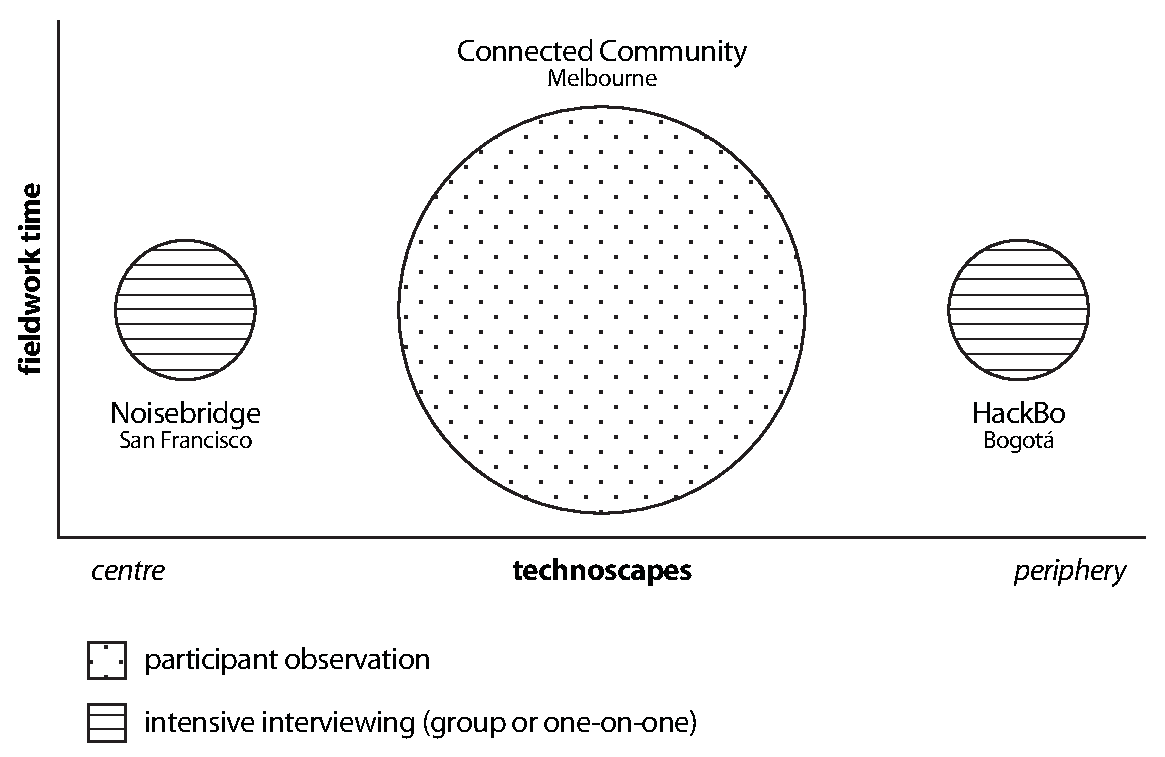
\includegraphics[scale=0.65,natwidth=10pt,natheight=1pt]{confirmation-report/graphs/methodology01.pdf}
	\caption[Synthesised Methodological Approach]{Synthesised methodological approach}
	\label{methodology_graph}
\end{figure}
%\end{center}


\subsubsection{Centre: \textit{Noisebridge} in San Francisco}

Noisebridge in San Francisco is one of the most prominent hackerspaces ---one that has served as a model for several others. Two main reasons make Noisebridge particularly noteworthy. First, it was one of the first original American spaces, founded by Mitch Altman, a well-known hacker who came up with the idea after his visit to the 2007 Chaos Communication Camp, a yearly hacker convention held in Germany\footnote{Section \ref{history} offers details on the conference's organisers: the Chaos Computer Club, a renowned hacker group.}. A piece on \textit{Wired} magazine details the genesis of Noisebridge, as well as American hackerspaces in general:

\begin{quote}
While many movements begin in obscurity, hackers are unanimous about the birth of U.S. hacker spaces (sic): August, 2007 when U.S. hackers Bre Pettis, Nicholas Farr, Mitch Altman and others visited Germany on a geeky field trip called Hackers on a Plane. \citep{tweney09}
\end{quote}

The second ---and most important reason for Noisebridge's notoriety is its location. As mentioned in section \ref{intro}, the origin of Silicon Valley as a central technological hub is closely tied to a group of early pioneers and the ever favourable influence of Stanford University and the U.S. Military \citep{lee00}. Today, and despite its well-known ups and downs, it is perhaps the most influential IT hub in the world, largely responsible for the technology-driven economic booms of the 1980s and 1990s in the United States \citep{bresnahan04}.

In curious contrast to this image of hi-tech behemoth, the Bay area at large has historically presented itself as a Mecca for countercultural movements at least since the 1950s, having served as base for the artists of the so-called \textit{San Francisco renaissance}, as well as becoming a centre for west coast beat poets, hippies, politically-aware students, radicals, dissidents, gays and a plethora of colourful characters.

Noisebridge's appeal thus lies in the fact that it is caught in the midst of the duality between the entrepreneurs and the bohemians: some of its members have long-standing careers in the Valley's tech industry, others have artistic or political backgrounds, while a special few seem to slide naturally between the two worlds. Altman himself is somewhat of a hippie and a pioneer of virtual reality technologies, having founded a company called 3ware\footnote{See \texttt{http://www.slideshare.net/maltman23}.}. Noisebridge's over 150 members range from professional programmers, to artists, activists and designers. It also has the dubious honour of counting Jacob Appelbaum (the most prominent American Wikileaks associate) as a founding member. Appelbaum has been the subject of several news reports lately, due to Wikileaks' spotlight, his relationship with Julian Assange \citep{rich10} and the continued harassment he has been subjected to by U.S. government officials \citep{mills10}.

\subsubsection{Periphery: \textit{HackBo} in Bogot\'{a}}

Some 6,000 kilometres south-east of San Francisco is HackBo, Bogot\'{a}'s own hackerspace. HackBo was founded in 2010 after three failed attempts to organise what was, until then, a loosely-tied community of mostly free and open source software hackers stemming from the country's public universities \citep{arizmendi11}. HackBo currently counts 15 fee-paying members and a larger number of associates\footnote{See \texttt{http://goo.gl/egzqK}.}, having now become a consolidated space, thanks in part to a strategic alliance with an already existing cultural centre, \textit{El Eje}\footnote{See \texttt{http://goo.gl/WXcTA}.} (The Axis), with which it shares a common habitat ---a house located in the city's university district. HackBo's members describe their space as an ``open community lab'' \citep{uribe11} where everybody is welcome to share their experiences and knowledge and to learn about computer languages and hardware hacking. 

HackBo was modelled after Hacker Dojo, another iconic American space founded by Lee Felsenstein\footnote{Felsenstein is a long-standing and well-known hacker, former moderator of the Homebrew Computer Club. See \citet{levy84} for more information.}. In terms of activities, it follows many of the same trends as other hackerspaces around the world: electronics tweaking, open source software and crafts, yet, for the purposes of my study, HackBo offers a very interesting opportunity.

Unlike the United States and Australia, whose budget for research and development is in the billions of dollars and represent relatively high percentages of their GDP\footnote{United States: 395.8 Billion, 2.8\% of GDP in 2010. Australia: 15.3 Billion, 1.8\% of GDP in 2010 \citep{wadsworth10}.}, Colombia occupies a humble fifty-second place, having invested about 600 million U.S. Dollars in 2007, only around .16\% of its GDP \citep[p.82]{unesco10}. Yet, there are perceivable cues that suggest change. Juan Manuel Santos, the recently elected President released an ambitious four-year plan for IT infrastructure immediately after reaching his position. The plan calls for an aggressive strategy to widen broadband usage and coverage in the country with special emphasis in depressed and remote regions, while promoting incentives for skills development and IT related business activities, particularly software development \citep{molano11}. 

Despite this ambitious push, which also includes the institution of three new IT research centres, there is still a relative scarcity of formal research entities in the country, a fact that raises the question as to whether or not hackerspaces can fulfil that role with some degree of success, either by positioning themselves as informal but effective research centres or by providing much-needed knowledge and skills to future researchers. 

Colombia's current stance with regards to ICT, combined with its unique cultural and social conditions, make HackBo attractive as a vehicle through which to study how environmental nuances influence learning and technological development inside hackerspaces.

\subsection{Research Strategy}
\label{strategy}

Ethnographic participant observation will be my primary research method, complemented by in-depth interviews at hackerspaces overseas. I intend to collect a substantial amount of data and to reach major preliminary conclusions before undertaking any research outside of Australia, the intention being to use interview data from overseas to test for representativeness and generalisability (as well as deviations) by contrasting it against the original, more comprehensive sample, hoping to verify and evaluate what should by then be a well-developed, yet early analysis.

I intend to spend a considerable amount of time amongst Melbourne hackers, assuming the role of a participant observer, regularly attending the Connected Community's weekly Tuesday meetings as well as some of the more informal weekend ``hang-out'' sessions. Tuesday meetings are of a formal nature and highly attended (thus ideal for performing Interaction Ritual Theory analysis), while the more spontaneous weekend meetups are somewhat more intimate and will hopefully provide insight into power relations, conflict and other intimate phenomena.

In attempting to work within the boundaries of my theoretical foundation, I have identified key elements on which to focus, hoping to find patterns and consistent behaviours that will subsequently lead to deep and hopefully fruitful analysis. While my intention is to gather data for all chapters in a concurrent manner, I will focus my observations sequentially in the same order as my three core chapters so as to build upon them as the work progresses. Outlined below are these main focal elements.

\subsubsection{Core 1: Applying Interaction Ritual Theory}

\begin{itemize}
  \item Identification of specific hacker rituals as well as their nature (formal, natural) and degree of success (successful, failed, empty, forced).
  \item Identification of ritual ingredients and outcomes in the context of hackerspaces --- \citet[p.41]{collins04} describes well-delineated causes and consequences of IRT. I will attempt to spot such factors in rituals held in hackerspaces, placing added emphasis in co-presence and barriers (ingredients) and symbols and negotiated morality (outcomes).
  \item Identification of key situations leading to ``symbolisation'' and the establishment of sacred objects.
\end{itemize}

\subsubsection{Core 2: Applying Legitimate Peripheral Participation}

\begin{itemize}
  \item Identification of a clear power structure in the context of LPP's examination of the duality between newcomers and old-timers and the prior analysis of IRT's sacred objects.
  \item Identification of instances of negotiated meaning and common concern. Similarly to Polanyi, \citeauthor{lave91} argue that knowledge is partly negotiated within a group. Within hackerspaces, analysis of this common meaning could be especially fertile, particularly in shedding light on the processes of learning and participation.
  \item Identification of motivation factors leading to the transition from peripheral to full participation within hackerspaces.
\end{itemize}

\subsubsection{Core 3: Applying Cognitive Change}

\begin{itemize}
  \item Identification of problem selection in the context of prior analysis of symbolisation (core 1) and negotiated meaning (core 2). Cognitive Change Theory places problem-solving at the centre of technological advance\footnote{It should be noted that the concept of problem-solving, according to the author, is indeed a broad one, involving not only ``utilitarian'' activities but also aesthetic and intellectual ones \citep[p.84]{laudan84}.}, thus the nature of problem selection becomes especially meaningful in understanding how technology flourishes in hackerspaces.
  \item Categorisation of types of problems solved by hackers within the CCT system.
  \item Identification of the effects of the ``environment'' as described by \citet[p.101]{laudan84} in relation to technological production in hackerspaces, considering prior analysis of settings and rituals. Also, identification of potential ``niche-isation'' in different hackerspaces and the determining factors in this process.
\end{itemize}

It is worth mentioning that I intend to conduct all my research overtly, with full disclosure to the community. I have already engaged some members of Connected Community at a personal level, yet all official data collection will begin only after gaining approval from the Monash University Human Research Ethics Committee (MUHREC). I should also note that I am already acquainted with the process of gaining ethics approval and performing research within the committee's guidelines as a result of having chosen similar methods for my Master's thesis. Section \ref{timeline} specifies my timeline for gaining ethics approval and undertaking participant observation at Connected Community.


\subsection{Data and Data Analysis}

Fieldwork at Connected Community in Melbourne will be documented primarily with the aid of fieldnotes, following \citepos{schatzman73} note-taking method. Summarily, the procedure involves labelling notes into three categories: Observational (ON), Theoretical (TN) and Methodological (MN). At a later stage, the notes are further categorised into logical thematic packages and complemented by analytic memos that serve as more explicit and elaborated theoretical notes. As noted earlier, my observations will take place overtly so I expect to be able to take ``jotted notes'' \citep[p.90]{lofland95} on the spot, transforming them to ``full fieldnotes'' at a later time. 

While fieldnotes seem to be the data-gathering method of choice for social scientists at large \citep{silverman00,lofland95,schatzman73}, I share \citepos{perakila97} concerns regarding their reliability. At best, fieldnotes provide a mediated account of events, filtered by the researcher's own points of view or interpretations. At worst, they can reflect erroneous observations and lead to mistaken conclusions. Thus, I will attempt to simultaneously collect raw data in the form of audio or video recordings to the extent to which such recordings are logistically, socially and ethically admissible.

For the purposes of interviewing, audio recordings alone will be the method of choice. Interviews conducted for my Master's thesis provided me with some methodological experience in conducting and logging sessions. My method involves taking carefully annotated notes prior to transcribing. Much like the fieldnote model described above, the notes are categorised and, more importantly, accompanied by a detailed, time-coded guide by which one can easily refer back to the original data.

Moreover, I seek to analyse all my qualitative data using \citepos{miles84} method, by means of three concurrent flows of activity: \textit{reduction}, whereby one selects, focuses and simplifies raw data, \textit{display}, involving assembling information so that it allows for ``conclusion drawing and action taking'' (matrices, graphs, networks) and \textit{conclusion/verification}, in which one connects causes and propositions in order to infer and determine. I realise that data coding can be an extremely laborious process, so my overall timeline for the completion of this project (see Section \ref{timeline}) accounts for these steps.

\subsection{Potential Woes}

Realising that there is no such thing as a perfect methodological design, or a one-size-fits-all solution, I consider the task of identifying potential shortcomings with the proposed research design a mission-critical one. This section attempts to provide preliminary reflections on potential shortcomings. It also offers possible solutions and/or counter-arguments.

\begin{list}{\labelitemi}{\leftmargin=0em}

\item[] \textbf{Familiarity with the setting}. While prior contact with hackers and relatively good knowledge about their social etiquette and practices is almost certainly a good thing, it also carries with it the risk of making the researcher ``feel too comfortable''. \citet{hammersley90}, seems to agree by arguing that ``when a setting is too familiar, the danger of misunderstanding it is especially great''. It is thus important not to take anything for granted and to attempt to disregard previous facts or assumptions that are the result of prior experience. As such, making a conscious effort to enter the field without any biases or preconceptions is crucial.

Under this same category, one can find the risk of developing over-rapport with research subjects. Familiarity and shared values can stop a researcher from evaluating his or her settings critically. Establishing rapport is an ever-present recommendation in fieldwork guides, yet the risk of over-sympathising with members of the communities under study can result in lack of critical judgement. On the topic, \citet{roberts94} asks: ``how does one, whose self interests are foremost in beginning an examination of a social world, hope to remain objective enough to command a claim of validity from his audience?''. I do not believe there is a straightforward answer to that question, yet I am convinced that active and deliberate steps must be taken in order to prevent the loss of a researcher's independence and capacity for critical inquiry.

\item[] \textbf{Under-analysis of data}. Having chosen to study multiple fields, I run the risk of either collecting too much or too little data for any one of them. I have considered this possibility and attempted to minimise it by selecting specific (and meaningful) events to assist to while performing participant observation in Melbourne. With that same frame of mind, I have decided to limit fieldwork for my other two sites so as to only seek to identify similarities and divergences from tendencies already observed in Melbourne. This will hopefully provide me with a reasonable volume of data ---one that aids in reaching accurate findings without becoming overwhelming. Needless to say, this potential catch will also be considered when determining the number of interviews to be conducted at the two hackerspaces overseas.

\item[] \textbf{Multiple methods} \citeauthor{silverman00} warns about possible complications stemming from the use of multiple research methods: ``multiple methods may tempt novice researchers to move to another dataset when they are having difficulties in analysing one set of material'' \citep[p.134]{silverman00}. I share the author's concern, yet I view my methods as complementary. In essence, I will avoid turning to one set of data when the other does not fit. Instead, I will only use interview data to explicitly contrast existing findings that are the product of previous fieldwork in Melbourne.

\end{list}

By identifying potential problems with my methodology before they happen, I aim to minimise their impact and to plan out possible solutions or alternative methods if needed. I consider this section to be nothing more than a work in progress, in the sense that the above list will be extended, developed and revised as this work moves forward. 


\subsection{Some Thoughts on Financing and Logistics}
\label{budget}

This project is, by design, ambitious in nature. Not only is it broad in scope, but it also considers fields separated by great distances. As exciting as this sounds, its logistics can indeed become a cause for concern for a single PhD candidate with a moderate budget. Thus, securing proper financing has become an on-going priority. 

I intend to apply for a Postgraduate Travel Grant to conduct fieldwork\footnote{See \texttt{http://goo.gl/OwtyD}.}. As mentioned in section \ref{methods}, my choices of overseas hackerspaces have also been shaped by my personal circumstances. I am a Colombian citizen from Bogot\'{a}. I have been acquainted with various members of the hacker community in that city for a number of years and personally know at least one of the members of HackBo. This will reduce my barriers of entry to the site in terms of time and resources, while allowing me to cut my travel expenses by having a place to stay while I conduct my research. Moreover, due to the nature of international flight hubs, the simplest, most cost-effective way for me to fly to Bogot\'{a} is by connecting flights at the Los Angeles Airport in California. As a result, the logistics of my research at Noisebridge will be greatly minimised, as my stay in San Francisco will be relatively simple to arrange.

In light of the fact that time spent overseas will be short, I cannot engage in the same type of long-term participant observation I intend to conduct in Melbourne. Consequently, I have opted to adopt intensive interviewing as my main research method at these locations. Much like \citet{lofland95}, I do not view intensive interviewing as a substitute for participant observation. Rather, I see both methods as being complementary and appropriate for each of my circumstances, as I intend to build upon previous findings at these locations.

Naturally, much if not all of the preparatory work for these interviews will take place in Melbourne. I intend to contact members of both hackerspaces immediately after gaining ethics approval, well in advance of my trip. Having been a subscriber to both Noisebridge's and HackBo's public email lists since December 2010, I expect to be able to identify key members and to approach them prior to reaching my destinations.



%Furthermore, fieldwork will draw upon the work of burrell09, who views the ethnographic field as a ``cultural network'' composed of ``spaces, people and objects'' [p.189]burrell09 made up of multiple sites (some physical, some mediated) that ultimately converge into a single unit, much like \citepos{appadurai96} multiple \textit{scapes} represent a single cultural flow or Manuel Castells' view that ``society'' and ``network'' are increasingly fusing [p.65]lovink03.
